\documentclass[First Project.tex]{subfiles}
\begin{document}

\subsection{ Μέθοδος \textlatin{\textbf{Gauss-Seidel}} }

Η μέθοδος \textlatin{\textbf{Gauss-Seidel}} αποτελεί μία επαναληπτική μέθοδος επίλυσης γραμμικών συστημάτων της μορφής \textlatin{\textbf{Ax = b}},
όπου $Α$ τετραγωνικός πίνακας $n \times n$. Χρησιμοποιείται συνήθως σε αραιά συστήματα όπου και έχει καλύτερη απόδοση από την μέθοδο της 
\textlatin{\textbf{PA = LU}} αποσύνθεσης. Η συνάρτηση που έχει υλοποιηθεί στο αρχείο \textlatin{\textbf{gauss\_seidel.py}} υλοποιεί τον 
παρακάτω αλγόριθμο :
\begin{itemize}
    \item Για κάθε γραμμή $i$ του πίνακα $Α$ υπολόγισε το άθροισμα των τιμών των μεταβλητών που έχουν ανανεωθεί σε αυτό το βήμα, για τις 
        μεταβλητές που δεν έχουν ανανεωθεί ακόμα χρησιμοποιήσε τις τιμές τους από την προηγούμενο βήμα.
    \item Ανάθεσε στο στοιχείο $x_{i}$ την τιμή 
    \begin{equation*}
            \frac{1}{A_{ii}}(b_{i} - \sum_{j=1}^{i-1} a_{ij}x_{j} - \sum_{j=i+1}^{n} a_{ij}x_{j}), 
    \end{equation*}
    όπου $\sum_{j=1}^{i-1} a_{ij}x_{j}$ το άθροισμα των τιμών των μεταβλητών που έχουν ανανεωθεί σε αυτό το βήμα και
    $\sum_{j=i+1}^{n} a_{ij}x_{j}$ αυτών που δεν έχουν ανανεωθεί.
    \item Συνέχισε την παραπάνω διαδικασία μέχρι να υπολογιστεί η λύση με την επιθυμητή ακρίβεια.
\end{itemize}

Πιο συγκεκριμένα, η συνάρτηση \textlatin{\textbf{gauss\_seidel}} δέχεται ως παραμέτρους τον πίνακα \textlatin{A}, το διάνυσμα \textlatin{b} και
την επιθυμητή ακρίβεια και επιστρέφει την λύση του συστήματος $x$. Το \textlatin{\textbf{default}} όρισμα \textlatin{\textbf{eps}} έχει την 
τιμή που χρειάζεται για ακρίβεια \textbf{4} δεκαδικών ψηφίων. Αρχικά, η συνάρτηση πραγματοποιεί τις κατάλληλες αρχικοποιήσεις των διανυσμάτων
$x$ και \textlatin{previous\_x} για να μπορεί να υπολογισθεί η ακρίβεια της λύσης καθώς και δημιουργεί και ένα αντίγραφο του πίνακα $Α$ έτσι ώστε να μην
πραγματοποιήσει καμία αλλαγή στον πίνακα που πήρε σαν όρισμα. Στην συνέχεια, για κάθε γραμμή $i$ του πίνακα $Α$ υπολογίζει τον αντίστροφο του
συντελεστή της μεταβλητής $x_{i}$ και το άθροισμα των τιμών των μεταβλητών. Για τις μεταβλητές που έχουν ανανεωθεί σε αυτό το βήμα 
χρησιμοποιεί τις νέες τιμές τους, ενώ γι' αυτές που δεν έχουν ανανεωθεί τις τιμές τους από το προηγούμενο βήμα. Έπειτα, αλλάζει τις τιμές του
διανύσματος \textlatin{previous\_x} και την τιμή του διανύσματος $x$ σύμφωνα με την τιμή που αναφέρθηκε παραπάνω και ελέγχει αν η εκτίμηση της λύσης 
έχει βρεθεί με την επιθυμητή ακρίβεια \textlatin{\textbf{eps}}. Η ακρίβεια υπολογίζεται ως προς την άπειρη νόρμα του σφάλματος στην λύση.
Τέλος, αναφέρεται ότι αν ο $Α$ έχει κυριαρχική διαγώνιο η μέθοδος συγκλίνει με οποιοδήποτε αρχικό διάνυσμα $x_{0}$, η συνάρτηση ξεκινάει από
το μηδενικό διάνυσμα μήκους $n$. Στην συνέχεια παρουσιάζεται η λύση του συστήματος που ζητείται για $n=10$ και $n=10000$ με το οποίο τελειώνει 
αυτή η παράγραφος. Το σύστημα είναι το παρακάτω 
\begin{center}
    $ \begin{pmatrix}
        5 & -2 &  &  &  \\
        -2 & 5 & -2 &  &  \\
         & \ddots & \ddots & \ddots &  \\
         &  & -2 & 5 & -2 \\
         &  &  & -2 & 5
    \end{pmatrix} 
    \begin{pmatrix}
        x_{1} \\
        x_{2} \\
        x_{3} \\
        \vdots \\
        x_{n}
    \end{pmatrix} = 
    \begin{pmatrix}
        3 \\
        1 \\
        \vdots \\
        1 \\
        3
    \end{pmatrix}$
\end{center} 

Για την λύση του παραπάνω συστήματος αρχικά δημιουργούμε τον πίνακα $Α$ με παρόμοιο τρόπο όπως στην παράγραφο \textbf{4.1} και καλούμε την 
συνάρτηση \textlatin{\textbf{gauss\_seidel}} με όρισμα τον πίνακα $Α$ και το διάνυσμα $b$ από την οποία παίρνουμε τα εξής αποτελέσματα ( με 
ακρίβεια 4 δεκαδικών ψηφίων ):
\begin{figure}[h!]
    \centering
    \captionsetup{justification=centering}
    \begin{center}
        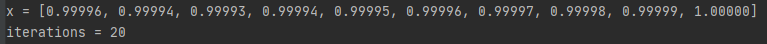
\includegraphics[scale=0.65]{exercise_3_gauss_seidel_solution_n_10.png}    
        \caption{ Λύση του συστήματος για $n=10$ }
    \end{center}
\end{figure} 

Ώπου παρατηρούμε ότι τα $x_{i}$ με ακρίβεια 4 δεκαδικών είναι \textbf{0.9999} και ότι χρειάστηκαν 20 επαναλήψεις για να συγκλίνει
ο αλγόριθμος με την επιθυμητή ακρίβεια. Για $n = 10000$ τα $x_{i}$ είναι και πάλι \textbf{0.9999} και χρειάστηκαν 23 επαναλήψεις για να 
συγκλίνει ο αλγόριθμος με την επιθυμητή ακρίβεια ( Η λύση δεν εμφανίζεται για ευνόητους λόγους ).
\newpage
\end{document}